\begin{figure}[H]
\begin{center}
  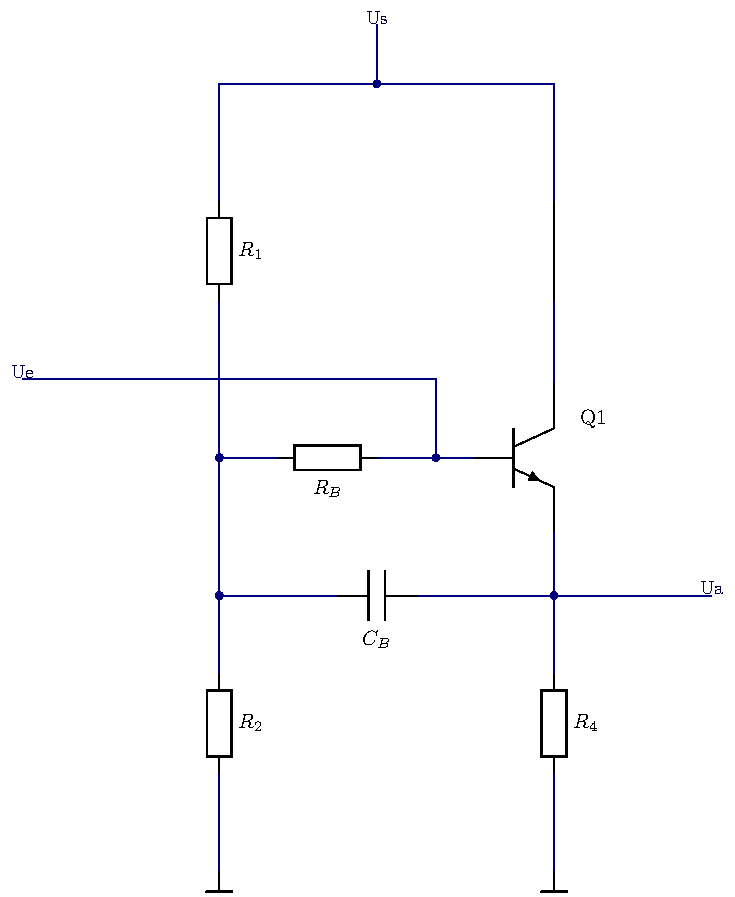
\includegraphics[width=0.618\textwidth]{circuits/bootstrap.pdf}
  \end{center}
\end{figure}


Bootstrapping ist eine Art der positiven Rückkopplung mit dem Ziel den
Eingangswiderstand der Schaltung zu erhöhen.

Bei der Kollektorschaltung kann
dies von Vorteil sein, um den Einsatz als Impedanzwandler zu verbessern.
Zur Kopplung wird ein Kondensator $C_B$ zwischen Ausgang und Basis geschaltet.
Eine schnelle Änderung des Ausgangssignals wirkt sich durch den Kondensator
ebenso auf den Eingang/die Basis aus, wobei beachtet werden muss, dass dieser so
dimensioniert ist, dass er bei der kleinsten Signalfrequenz einen Kurzschluss
darstellt.

Da die Verstärkung der Kollektorschaltung
kleiner als eins (z.B. 0.97) ist, beginnt der Verstärker nicht zu schwingen, wie es sonst
bei Mitkopplungen üblich wäre. Das Eingangssignal tritt mit leicht geringerer
Amplitude im Eingangskreis erneut auf, sodass der Strom durch den Widerstand
$R_B$, welcher den Basisspannungsteilerpunkt mit der Basis verbindet, sehr
gering ist, wodurch der scheinbare Wert von $R_B$ erhöht wird.

Der effektive (Kleinsignal-) Wert von $R_B$ ist
\[R_{B,eff} = \frac{R_B}{1-V_u}\]